\section{Теорема о неявной функции.}
\subsection*{Подводочка под водочку.}
\begin{conj}
    Пусть $x \in \R^n, y \in \R^m$. 
    Тогда $(x, y) \in \R^{n + m}$.  
    То есть мы как бы склеиваем их в один большой вектор.
\end{conj}

\begin{notice}
    При применении линейного отображения не надо путать с билинейной формой, т.е. $\A(x, y)$ это применение линейного отображения к одному цельному вектору $(x, y)$.
\end{notice}

\begin{lemma}
    Пусть $\A : \R^{n + m} \to \R^n$ -- линейное отображение, т.ч. $\A(h, 0_m) = 0_n \Rightarrow h = 0_n$.
    \\ Тогда $\forall y \in \R^m$ уравнение $\A(x, y) = 0$ имеет единственное решение.
\end{lemma}
\begin{proof}
    Рассмотрим линейный оператор: \begin{gather*}
        \varphi: \R^n \to \R^n \\
        h \mapsto \A(h, 0)
    \end{gather*}
    \quad Докажем, что $\varphi$ -- биекция.
    Размерности у нас совпадают, поэтому достаточно проверить инъективность.
    Для инъективности же достаточно тривиальности ядра. 
    А это как раз и есть особенность нашего отображения: $\A(h, 0_m) = 0_n \Rightarrow h = 0_n$.

    \quad Вследствие линейности $\A(x, y) = 0 \Leftrightarrow \A(x, 0) = -\A(0, y)$.
    Так как $\varphi$ биекция, мы можем применить обратное отображение:
    \begin{gather*} 
        \varphi^{-1}(\A(x, 0)) = \varphi^{-1}(-\A(0, y)) \\
        x = \varphi^{-1}(-\A(0, y))
    \end{gather*}
    \quad Таким образом, при фиксированном $y$ мы однозначно находим $x$.
\end{proof}

Дальше наша глобальная цель будет состоять в том, чтобы понять, при каком условии уже нелинейные уравнения будут разрешимы.
Но пока что разберем простой пример.

\vspace*{5mm}

\textbf{Пример:}
Рассмотрим уравнение $x^2 + y^2 = 1$:
\begin{center}
    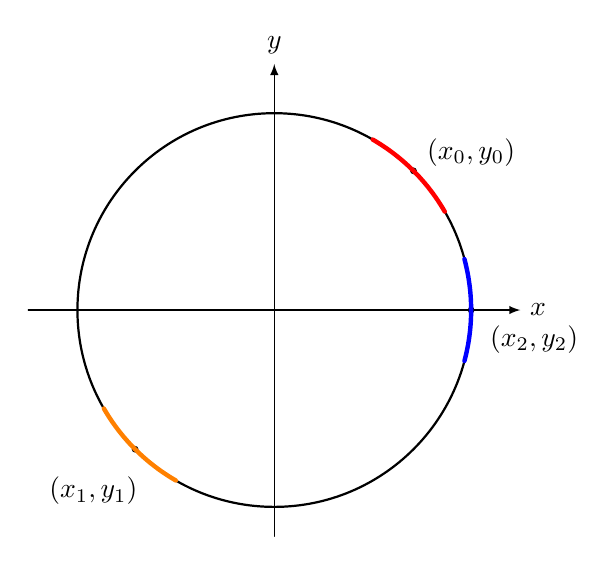
\begin{tikzpicture}[scale=2.5,cap=round,>=latex]
        % draw the coordinates
        \draw[->] (-1.25cm,0cm) -- (1.25cm,0cm) node[right,fill=white] {$x$};
        \draw[->] (0cm,-1.15cm) -- (0cm,1.25cm) node[above,fill=white] {$y$};

        % draw the unit circle
        \draw[thick] (0cm,0cm) circle(1cm);

        \filldraw[black] (45:1cm) circle(0.4pt)
                        (45:-1cm) circle(0.4pt)
                        (0:1cm) circle(0.4pt);

        \draw (1.32cm,-0.15cm) node(b) {$(x_2, y_2)$}
                        (1.0cm,0.8cm) node(a) {$(x_0, y_0)$}
                        (45:-1.3cm) node(c) {$(x_1, y_1)$};
                        
        \draw [red,ultra thick,domain=30:60] plot ({cos(\x)}, {sin(\x)});
        \draw [blue,ultra thick,domain=-15:15] plot ({cos(\x)}, {sin(\x)});
        \draw [orange,ultra thick,domain=210:240] plot ({cos(\x)}, {sin(\x)});
    \end{tikzpicture}
\end{center}
Если мы изобразим решения этого уравнения, то получится единичная окружность.
Зафиксируем на ней точку $(x_0, y_0)$. 
Если мы будем сдвигаться от нее немного влево и вправо, то у нас получится график функции.

Мы даже можем легко понять, как устроена эта функция: $g(x) = \sqrt{1 - x^2}$.
Так вот такая функция называется неявно заданной уравнением $x^2 + y^2 = 1$.

Если же мы зафиксируем точку $(x_1, y_1)$, то неявная функция примет вид $g(x) = -\sqrt{1 - x^2}$. 
А для точки $(x_2, y_2)$ это уже будет $h(y) = \sqrt{1 - y^2}$. 
Заметим, что для двух предыдущих точек мы также могли записать функцию для $y$.

%Теорема о неявной функции как раз и говорит о том, в каком случае мы можем написать неявную функцию для конкретной переменной в конкретной точке.

\begin{theorem} [о неявной функции]
    Пусть:
    \begin{itemize}
      \item $f \colon D \to \R^n$, где $D \subset \R^{n + m}$ и $D$ --- открыто.
      \item $f$ --- непрерывно дифференцируема.
      \item $f(a, b) = 0$ для какой-то точки $(a, b) \in D$.
      \item $A \coloneqq f'(a, b)$ и $A$ удовлетворяет условию $A(h, 0) = 0 \implies h = 0$.
    \end{itemize}
    Тогда существует окрестность $W$ точки $b$ и единственная функция $g\colon W \to \R^n$ такая, что~$g$ непрерывно дифференцируема, $g(b) = a$ и $f(g(y), y) = 0\;\; \forall y \in W$. 
    

    \textit{Смысл такой, что если у нас есть вектор $(a, b)$, который является решением уравнения $f(a, b) = 0$, и матрица из производных обладает нужным свойством, то найдутся другие решения уравнения, 
    причем они будут описываться функцией $g$, принимающей последние $m$ координат и выдающей по ним первые $n$ координат.
    Эта функция $g$ как раз и будет неявной.
    Можно провести аналогию с решением системы линейных уравнений: 
    у нас есть $m$ свободных неизвестных и $n$ зависимых.}
\end{theorem}
  \begin{proof}
    Заведем вспомогательную функцию:
    \begin{equation*}
      \begin{gathered}
        F\colon D \longrightarrow \R^{n + m} \\
        F(x, y) \coloneqq (f(x, y), y)
      \end{gathered}
    \end{equation*}
    Докажем, что получившаяся функция непрерывно дифференцируема. Во-первых заметим, что из непрерывной дифференцируемости $f$ следует, что:
    \begin{equation*}
      f(a + h, b + k) = \underbrace{f(a, b)}_{0} + A(h, k) + \underbrace{r(h, k)}_{o(\|(h, k)\|)}
    \end{equation*}
    Тогда:
    \begin{gather*}
        \begin{split}
            F(a + h, b + k) &= (f(a+h, b+k), b+k) \\
            &= (f(a, b) + A(h, k) + r(h, k), b+k) \\
            &= (f(a, b), b) + (A(h, k), k) + (r(h, k), 0) \\
            &= F(a, b) + (A(h, k), k) + o(\| (h, k) \|)
        \end{split}    
    \end{gather*}
    
    При этом $(r(h, k), 0) = o(\| (h, k) \|)$ просто потому что $r(h, k) = o(\| (h, k) \|)$. То есть верна дифференцируемость, а непрерывность следует из того, что $A$ непрерывно зависит от точки(потому что $f$ непрерывна), а значит и в нашем случае будет верна непрерывность(это будет видно дальше, когда мы напишем явный вид $F'(a, b)$).
  
    Таким образом $F$ непрерывно дифференцируема и мы легко можем понять чему равно $F'(a, b)$. Посмотрев на второе слагаемое в разложении $F(a + h, b + k)$ легко видеть, что для каждого из $n~+~m$ базисных векторов, первые $n$ координат переходят в соответствующие $n$ координат их образов(по оператору $A$). При этом оставшиеся $m$ координат сохраняются(то есть в случае стандартного базиса равны нулю для первых $n$ векторов, и равны единице для оставшихся $m$ векторов):
    \begin{equation*}
      F'(a, b) =
      \begin{pmatrix}
        \multicolumn{2}{c}{A} \\
        0 & E_m
      \end{pmatrix}
    \end{equation*}
    \textit{Как и было замечено раннее, если матрица $A$ зависит непрерывно от точки $(a, b)$, то и вся матрица $F'(a, b)$ непрерывно зависит от точки $(a, b)$, просто потому что все остальные элементы матрицы это какие-то фиксированные числа.}
  
    Получили какое-то отображение, теперь давайте посмотрим на его ядро и поймем является ли наша матрица невырожденной. Пусть $(F'(a, b))(h, k) = 0$. Тогда:
    \begin{equation*}
      (F'(a, b))(h, k) = 0 \implies (A(h, k), k) = 0 \implies k = 0 \implies A(h, 0) = 0 \overset{\text{усл.}}{\implies} h = 0
    \end{equation*}
    Таким образом ядро тривиально, а значит матрица $F'(a, b)$ невырожденная.
  
    Значит по теореме об обратной функции $F$ локально обратима, то есть $\exists\; U$ --- окрестность точки~$(a, b)$, $V$ --- окрестность точки $F(a, b) = (0, b)$ и функция $G\colon V \to U$ обратная к $F$. Хотим показать, что
    \begin{equation*}
      G(z, w) = (\varphi(z, w), w)
    \end{equation*}
    Действительно, мы хотим, чтобы $F(G(z, w)) = (z, w)$, но $F$ сохраняет последние $m$ координат, поэтому последние $m$ координат у $G(z, w)$ также должны быть равны $w$. При этом $\varphi(z, w)$ это просто какая-то произвольная функция, про которую мы ничего не утверждаем, поэтому эта часть тоже очевидна верна. Тогда:
    \begin{equation*}
      \begin{cases}
        F(G(z, w)) = (z ,w) \\
        F(G(z, w)) = F(\varphi(z, w), w) = (f(\varphi(z, w), w), w)
      \end{cases}
      \implies f(\varphi(z, w), w) = z
    \end{equation*}
    Возьмем $W$ --- окрестность точки $b$ такую, что $\{0\} \times W \subset V$ --- разумеется такая есть, потому что $(0, b)$ лежит в $V$ с какой-то окрестностью. И пусть:
    \begin{equation*}
      \begin{gathered}
        g\colon W \to \R^n \\
        g(w) \coloneqq \varphi(0, w)
      \end{gathered}
    \end{equation*}
    Тогда заметим, что 
    \begin{equation*}
      F(a, b) = (f(a, b), b) = (0, b) \implies G(0, b) = (a, b) \implies (\varphi(0, b), b) = (a, b) \implies \varphi(0, b) = a
    \end{equation*}
    То есть $g(b) = a$. При этом $f(g(w), w) = f(\varphi(0, w), w) = 0$. Также легко видеть, что непрерывная дифференцируемость $g$ следует напрямую из теоремы об обратной функции. 
  
    Осталось доказать единственность, пусть это не так, тогда $g(y) \neq \widetilde{g}(y)$. Но 
    \begin{equation*}
      f(g(y), y) = f(\widetilde{g}(y), y) = 0
    \end{equation*}
    Тогда 
    \begin{equation*}
      F(g(y), y) = (f(g(y), y), y) = (0, y) = (f(\widetilde{g}(y), y), y) = F(\widetilde{g}(y), y)
    \end{equation*}
    Таким образом мы получили равные значения $F$ при разных значениях аргумента. Но $F$ --- биекция, а значит такого не может быть. Значит $g$ --- единственно.
  \end{proof}
  
  \notice \; Условие $A(h, 0) = 0 \implies h = 0$ означает следующее:
  \begin{equation*}
    A \begin{pmatrix}
      h \\ 0
    \end{pmatrix}
    =
    \begin{pmatrix}
      B & C
    \end{pmatrix}
    \begin{pmatrix}
      h \\ 0
    \end{pmatrix}
    =
    Bh
  \end{equation*}
  То есть условие на самом деле формулируется следующим образом: $Bh = 0 \implies h = 0$. А это верно тогда и только тогда, когда $\det B \neq 0$. Иными словами мы берем минор по первым $n$ координатам и говорим, что этот минор ненулевой.
  
  \notice \; Это условие также можно переформулировать для произвольных $n$ координат. Действительно, если $\rk A = n$, то существует какой-то невырожденный минор порядка $n$, а значит наша теорема применима к координатам, соответствующим этому минору.
  